\documentclass{article}
\usepackage{booktabs}
\usepackage{graphicx} % Required for inserting images
\usepackage{geometry}
\geometry{margin=0.7in}
\usepackage[T1]{fontenc}%
\usepackage[utf8]{inputenc}%
\usepackage{lmodern}%
\usepackage{textcomp}%
\usepackage{lastpage}%
\usepackage{pdflscape}%
\usepackage[table]{xcolor}%
\usepackage{amsmath}%
\usepackage{color}%
\usepackage{multirow}%
\usepackage{longtable}%
\usepackage{xcolor}%
\usepackage{tabularx}%
\usepackage{ltablex}%
\usepackage{subcaption} % For subfigures

%

\title{OPTIMIZATION REPORT}
\author{Statistical Arbitrage}
\date{04/04/2024}

\begin{document}

\maketitle

\section{Parameter Optimization Details}

The following table summarizes the parameters used in the optimization process, including their types, ranges, step sizes, and optimal values determined from the trials.

\begin{table}[h]
\centering
\caption{Parameter ranges and optimal values used in the optimization process.}
\label{tab:parameter_ranges}
\begin{tabular}{llrrrr}
\toprule
\textbf{Parameter} & \textbf{Type} & \textbf{From} & \textbf{To} & \textbf{Step} & \textbf{Optimal} \\
\midrule
estimation\_window & Integer & 40 & 80 & 10 & 40 \\
min\_trading\_days\_fraction & Float & 0.5 & 0.8 & 0.15 & 0.8 \\
top\_stocks & Integer & 3 & 9 & 3 & 6 \\
correlation\_threshold & Float & 0.3 & 0.6 & 0.3 & 0.6 \\
tier & Categorical & 1 & 4 & -- & 1 \\
first\_allocation & Float & 0.4 & 0.7 & 0.15 & 0.4 \\
adding\_allocation & Float & 0.2 & 0.3 & 0.1 & 0.2 \\
cluster & Int & 8 & 10 & 2 & 10\\
\bottomrule
\end{tabular}
\end{table}

\section{Optimization Results}

Figure~\ref{fig:optimization_plots} \textbf{Train Set}
\begin{figure}[h!]
\centering
\begin{subfigure}{0.48\textwidth}
    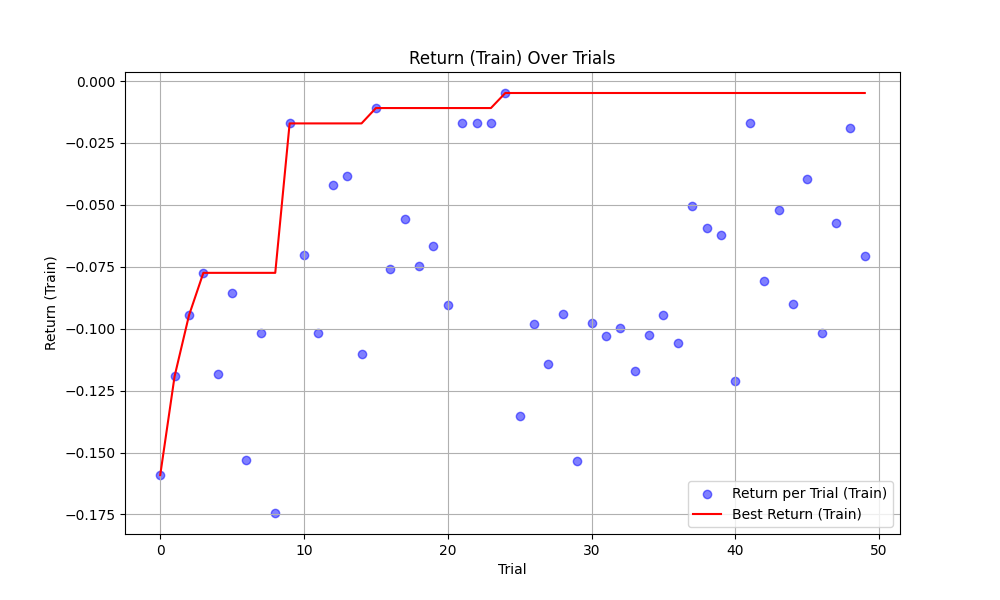
\includegraphics[width=\textwidth]{trial_return.png}
    \caption{Optimization history plot showing the annual return (train) value over trials.}
    \label{fig:optimization_history}
\end{subfigure}
\hfill
\begin{subfigure}{0.48\textwidth}
    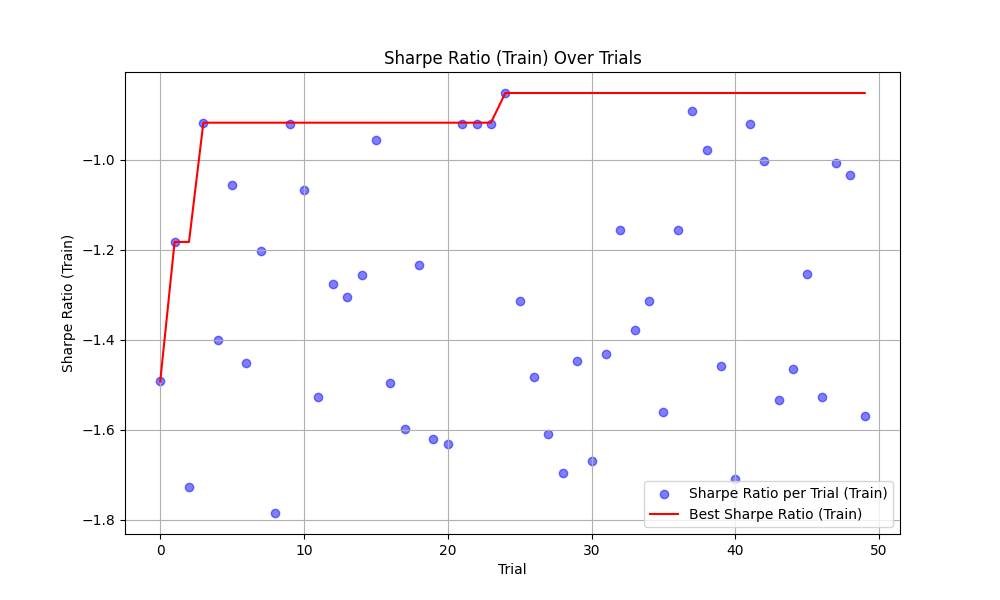
\includegraphics[width=\textwidth]{trial_shapre.png}
    \caption{Optimization history plot showing the sharpe (train) value over trials}
    \label{fig:parameter_importances}
\end{subfigure}
\caption{Visualization of the optimization process: (a) annual return and (b) sharpe.}
\label{fig:optimization_plots}
\end{figure}

Figure~\ref{fig:optimization_plots} \textbf{Test Set}
\begin{figure}[h!]
\centering
\begin{subfigure}{0.48\textwidth}
    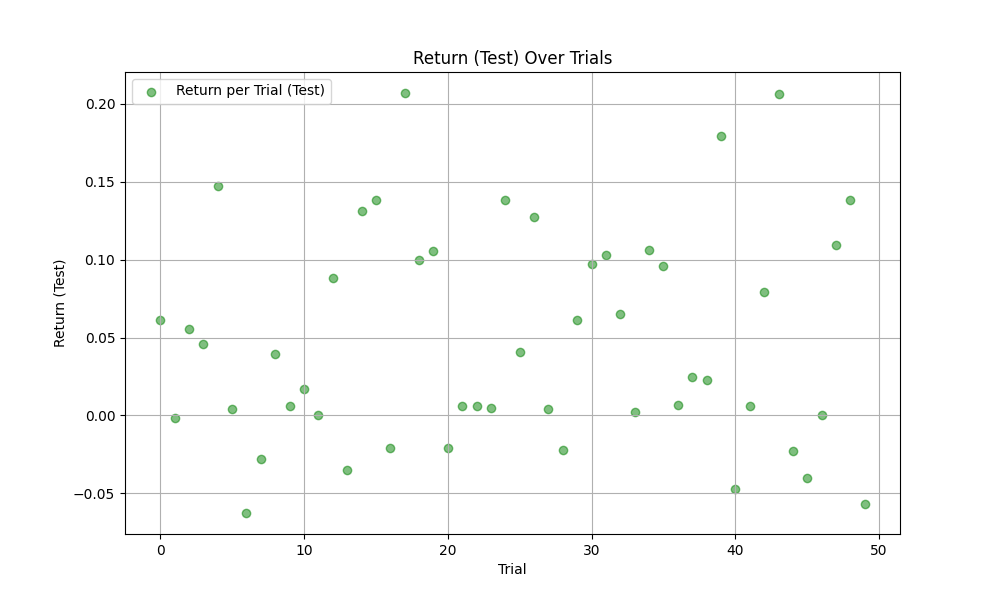
\includegraphics[width=\textwidth]{trial_return_test.png}
    \caption{Optimization history plot showing the annual return (test) value over trials.}
    \label{fig:optimization_history}
\end{subfigure}
\hfill
\begin{subfigure}{0.48\textwidth}
    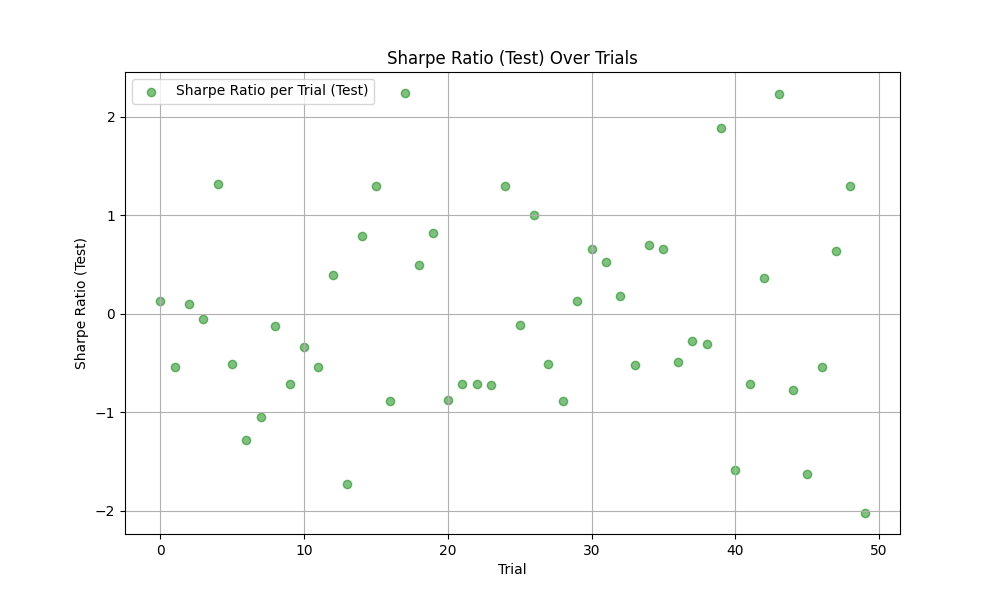
\includegraphics[width=\textwidth]{trial_sharpe_test.png}
    \caption{Optimization history plot showing the sharpe (train) value over trials}
    \label{fig:parameter_importances}
\end{subfigure}
\caption{Visualization of the optimization process: (a) return and (b) sharpe.}
\label{fig:optimization_plots}
\end{figure}


\end{document}
